\section{Resultados experimentales}

\subsection{Comparacion de rendimiento}

La Tabla~\ref{tab:performance} compara la ejecucion completa del proyecto en un nodo frente a la ejecucion completa en el cluster YARN de tres nodos. Se usa como referencia la ejecucion \texttt{all}, que incluye ETL, consultas SQL, regresion y clasificacion.

\begin{table}[H]
    \centering
    \caption{Comparacion de rendimiento mononodo vs. multimodo.}
    \label{tab:performance}
    \footnotesize
    \renewcommand{\arraystretch}{1.15}
    \begin{tabularx}{\textwidth}{
        >{\raggedright\arraybackslash}p{0.15\textwidth}
        >{\centering\arraybackslash}p{0.07\textwidth}
        >{\centering\arraybackslash}p{0.08\textwidth}
        >{\centering\arraybackslash}p{0.13\textwidth}
        >{\centering\arraybackslash}p{0.13\textwidth}
        >{\centering\arraybackslash}p{0.08\textwidth}
        X}
        \toprule
        \textbf{Ambiente} & \textbf{Nodos} & \textbf{Vcores} & \textbf{Memoria YARN} & \textbf{Tiempo} & \textbf{Speedup} & \textbf{Observacion} \\
        \midrule
        Mononodo local & 1 & 2 aprox. & N/A & 7 min 02.693 s & 1.00 & Ejecucion \texttt{local[*]} sobre archivo local. \\
        Multimodo YARN & 3 & 4 & 8 GB & 18 min 45 s & 0.38 & Ejecucion distribuida sobre HDFS; mayor overhead por YARN, HDFS, shuffle y VMs. \\
        \bottomrule
    \end{tabularx}
\end{table}

\begin{table}[H]
    \centering
    \caption{Asignacion de recursos observada durante una ejecucion distribuida.}
    \label{tab:resources}
    \footnotesize
    \renewcommand{\arraystretch}{1.15}
    \begin{tabularx}{\textwidth}{
        >{\raggedright\arraybackslash}p{0.13\textwidth}
        >{\centering\arraybackslash}p{0.11\textwidth}
        >{\centering\arraybackslash}p{0.10\textwidth}
        >{\centering\arraybackslash}p{0.10\textwidth}
        >{\raggedright\arraybackslash}p{0.17\textwidth}
        >{\raggedright\arraybackslash}p{0.15\textwidth}
        X}
        \toprule
        \textbf{Nodo} & \textbf{Mem. conf.} & \textbf{Vcores conf.} & \textbf{Cont.} & \textbf{Recurso asignado} & \textbf{Uso observado} & \textbf{Rol} \\
        \midrule
        \texttt{master} & 4096 MB & 2 & 2 & 2048 MB, 2 vcores & PMem aprox. 697 MB & Driver/ApplicationMaster y tareas. \\
        \texttt{slave1} & 2048 MB & 1 & 1 & 1024 MB, 1 vcore & PMem aprox. 171 MB & Worker. \\
        \texttt{slave-base} & 2048 MB & 1 & 1 & 1024 MB, 1 vcore & PMem aprox. 176 MB & Worker. \\
        \bottomrule
    \end{tabularx}
\end{table}


\begin{figure}[H]
    \centering
    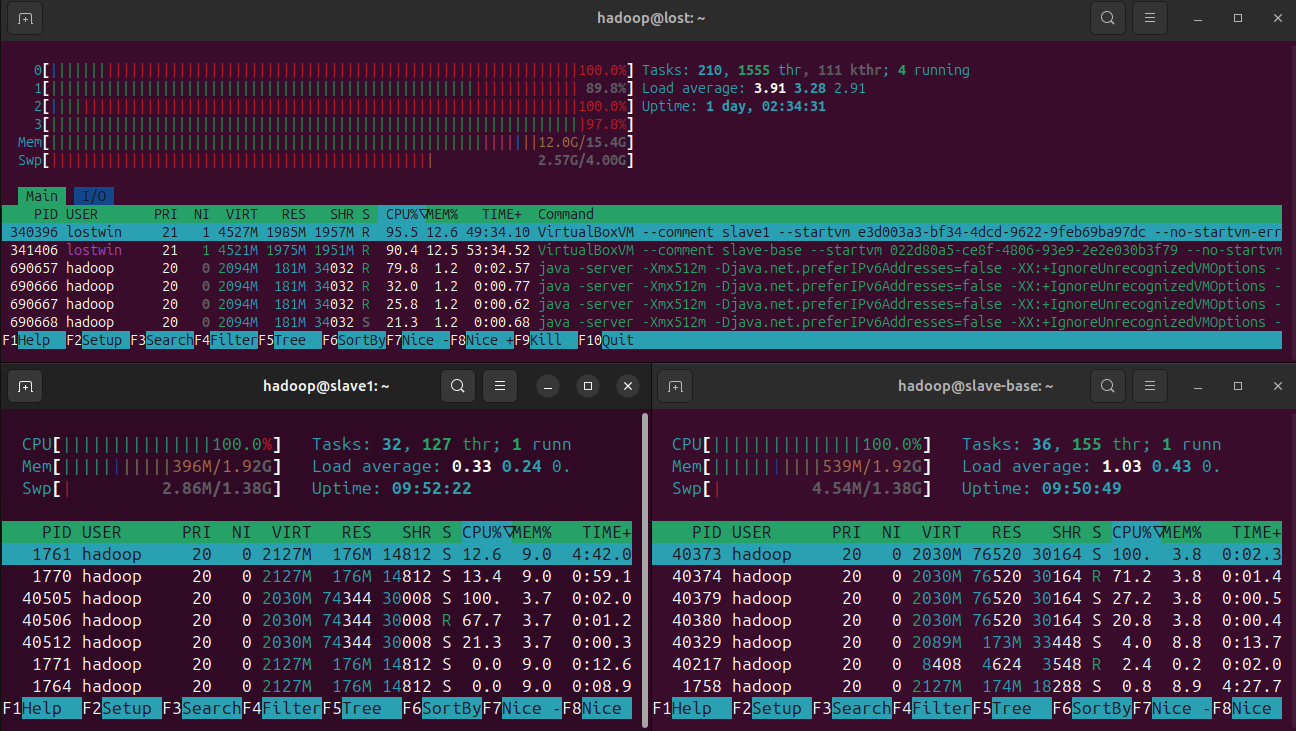
\includegraphics[width=\textwidth]{ImgNod1/Capturas_Rercursos_3nodo_en_vivo.png}
    \caption{Monitor de recursos por nodo durante la ejecucion: master, slave1 y slave-base.}
    \label{fig:htop-all}
\end{figure}

\subsection{Metricas de regresion}

\begin{table}[H]
    \centering
    \caption{Metricas de regresion: comparacion entre mononodo y cluster.}
    \label{tab:regression}
    \begin{tabular}{llrrrr}
        \toprule
        \textbf{Modelo} & \textbf{Ambiente} & \textbf{RMSE} & \textbf{MSE} & \textbf{MAE} & $\boldsymbol{R^2}$ \\
        \midrule
        MLPRegressor & Mononodo & 1352.55 & 1\,829\,399.43 & 281.91 & 0.2233 \\
        MLPRegressor & Cluster & 1384.64 & 1\,917\,232.43 & 284.91 & 0.2302 \\
        SVRegressor & Mononodo & 1430.10 & 2\,045\,182.64 & 232.98 & 0.1317 \\
        SVRegressor & Cluster & 1486.36 & 2\,209\,266.74 & 257.77 & 0.1130 \\
        \bottomrule
    \end{tabular}
\end{table}


En ambos ambientes el MLPRegressor obtuvo mejor RMSE y MSE que el SVRegressor. Los valores de $R^2$ son positivos pero moderados, lo que indica que las variables disponibles explican parte del comportamiento de \texttt{MONTO\_SERENAZGO}, aunque no capturan toda la variabilidad del cobro.

\subsection{Metricas de clasificacion}

\begin{table}[H]
    \centering
    \caption{Metricas de clasificacion: comparacion entre mononodo y cluster.}
    \label{tab:classification}
    \begin{tabular}{llrrrr}
        \toprule
        \textbf{Modelo} & \textbf{Ambiente} & \textbf{Accuracy} & \textbf{Precision} & \textbf{Recall} & \textbf{F1-score} \\
        \midrule
        RandomForest & Mononodo & 0.8614 & 0.8833 & 0.8614 & 0.8421 \\
        RandomForest & Cluster & 0.8593 & 0.8819 & 0.8593 & 0.8397 \\
        MLPClassifier & Mononodo & 0.7458 & 0.8367 & 0.7458 & 0.7615 \\
        MLPClassifier & Cluster & 0.7371 & 0.5433 & 0.7371 & 0.6255 \\
        \bottomrule
    \end{tabular}
\end{table}


Random Forest fue el modelo de clasificacion mas estable y con mejor F1-score. El MLPClassifier alcanzo desempeno superior al azar, pero fue mas sensible al entorno y a la separacion de datos; esto es esperable en una red pequena sin mayor ajuste de hiperparametros.

\begin{figure}[H]
    \centering
    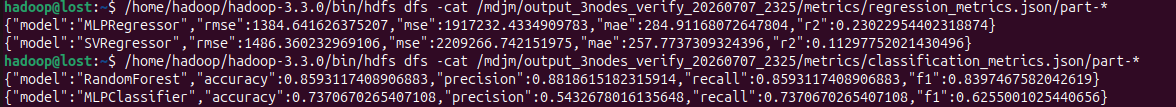
\includegraphics[width=\textwidth]{ImgNod1/Metricas_Regresion_Clasificacion.png}
    \caption{Metricas de regresion y clasificacion obtenidas en la ejecucion multimodo desde HDFS.}
    \label{fig:cluster-metrics-terminal}
\end{figure}
